\section{Overview}

Each strategy is optimized in stages. The stop-loss percentage is usually optimized first. All parameters that
are not optimized are kept fixed, either at their resting values or at values selected in previous stages.

The historical grids are evaluated directly on the real historical IS period. The synthetic grids are
evaluated on 50 synthetic paths generated from the same IS period, using the threshold-constrained
rolling-volatility GBM generator. The value reported at each synthetic grid point is the mean
performance across those paths. In every optimization plot, green indicates better values for the
metric shown and red indicates worse values.

The metrics reported throughout the chapter are net profit, average trade, Sharpe ratio, max DD, and
trades per year.

\section{Moving-average crossover optimization}

\subsection{Stop-loss stage}

The stop-loss percentage was optimized first, holding the rest of the parameters at their
resting values (\(fast\_len = 50\), \(slow\_len = 100\)). Figure~\ref{fig:mac-slpct} compares the
historical-IS sweep with the synthetic-path mean.

\begin{figure}[H]
    \centering

    \begin{tabular}{@{}cc@{}}
        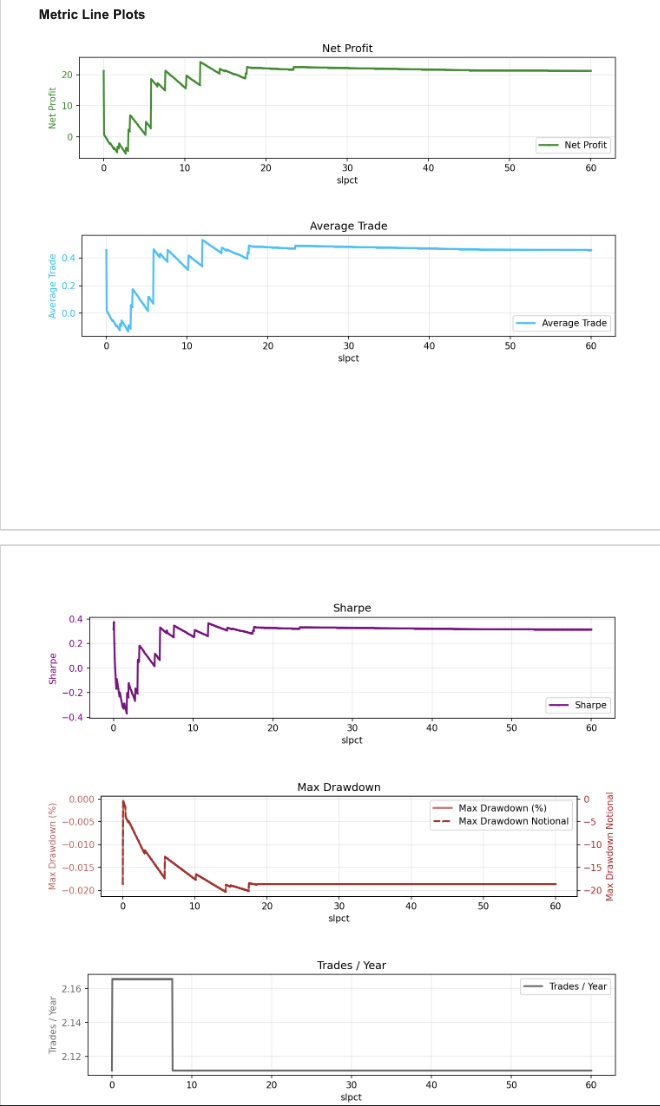
\includegraphics[height=0.44\textheight]{figures/opt/macross/slpct.png} &
        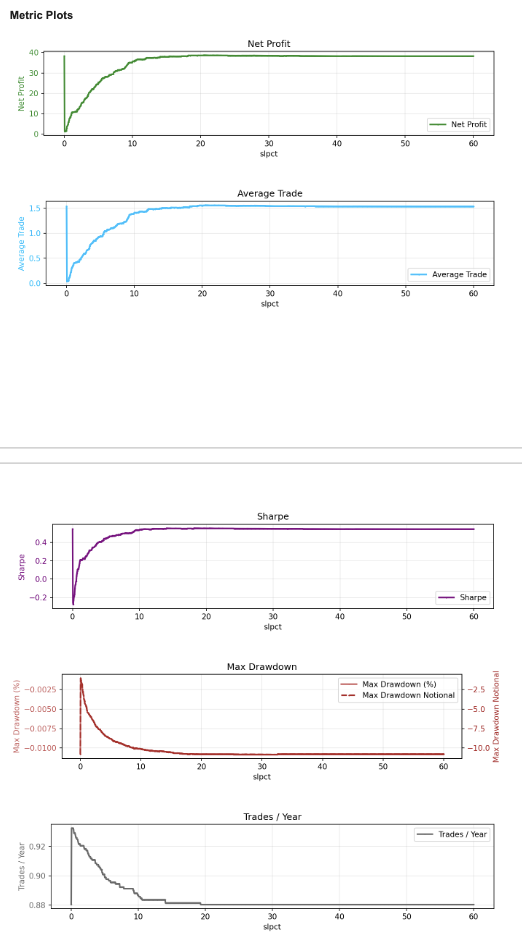
\includegraphics[height=0.44\textheight]{figures/opt/macross/syn_slpct.png}
    \end{tabular}

    \caption{Moving-average crossover: stop-loss optimization. Left: historical IS. Right: synthetic mean.}
    \label{fig:mac-slpct}
    \label{fig:mac-slpct-syn}
\end{figure}

The synthetic plot has a similar shape to the historical one, but it is smoother. This is expected,
since every point is averaged across 50 paths instead of being measured on one path only.

The stop-loss was left disabled (\(slpct = -1\)) for both the benchmark and the synthetic configuration
because short stop-loss values produced unstable results.

\subsection{Fast/slow length stage}

With the stop-loss disabled, the fast and slow moving-average lengths were optimized jointly.
Figures~\ref{fig:mac-mas}--\ref{fig:mac-ms2} compare the historical-IS grid with the synthetic-path
mean.

\begin{figure}[H]
    \centering

    \begin{minipage}{0.49\textwidth}
        \centering
        \textbf{Historical IS}\\[0.2em]
        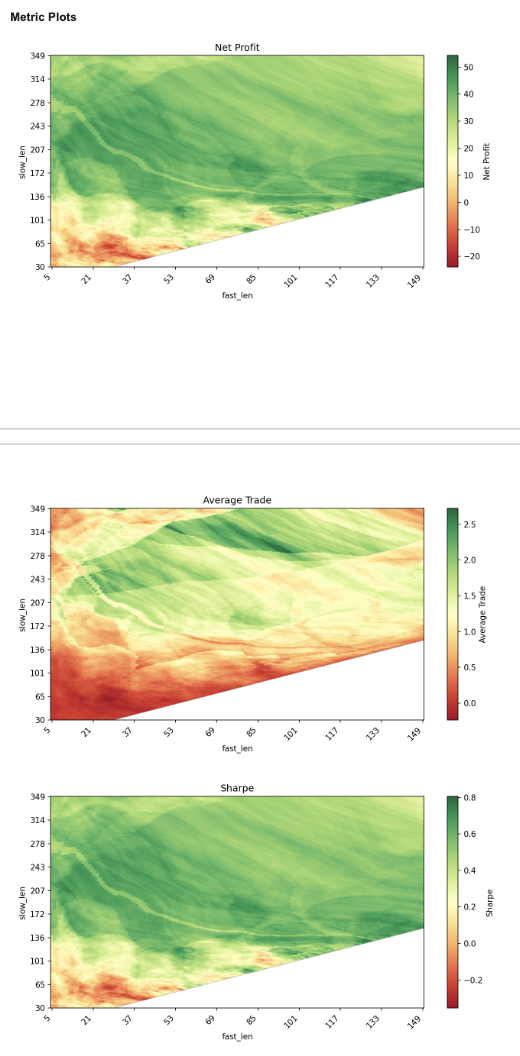
\includegraphics[width=\linewidth]{figures/opt/macross/mas.png}
    \end{minipage}
    \hfill
    \begin{minipage}{0.49\textwidth}
        \centering
        \textbf{Synthetic mean}\\[0.2em]
        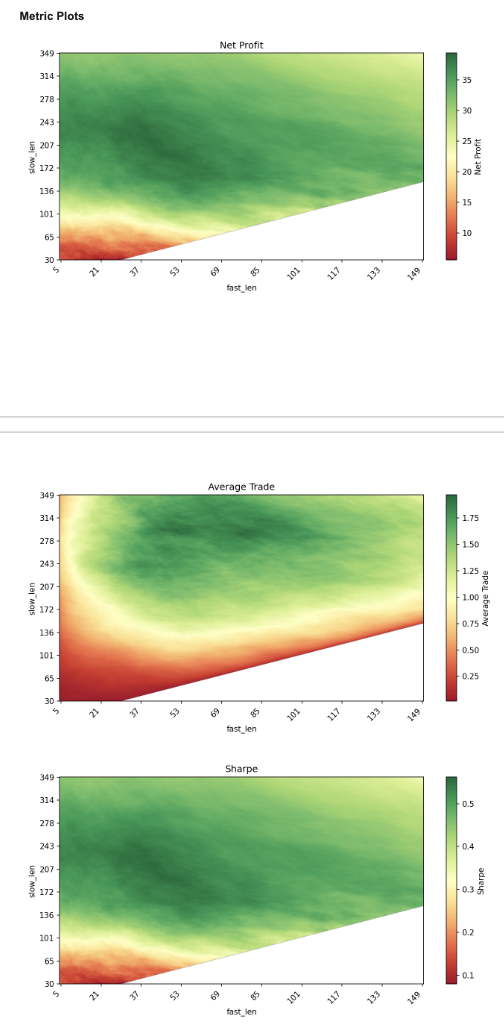
\includegraphics[width=\linewidth]{figures/opt/macross/syn_mas.png}
    \end{minipage}

    \caption{Moving-average crossover: first metric panel over the fast/slow length grid.}
    \label{fig:mac-mas}
    \label{fig:mac-syn-mas}
\end{figure}

\begin{figure}[H]
    \centering

    \begin{minipage}{0.49\textwidth}
        \centering
        \textbf{Historical IS}\\[0.2em]
        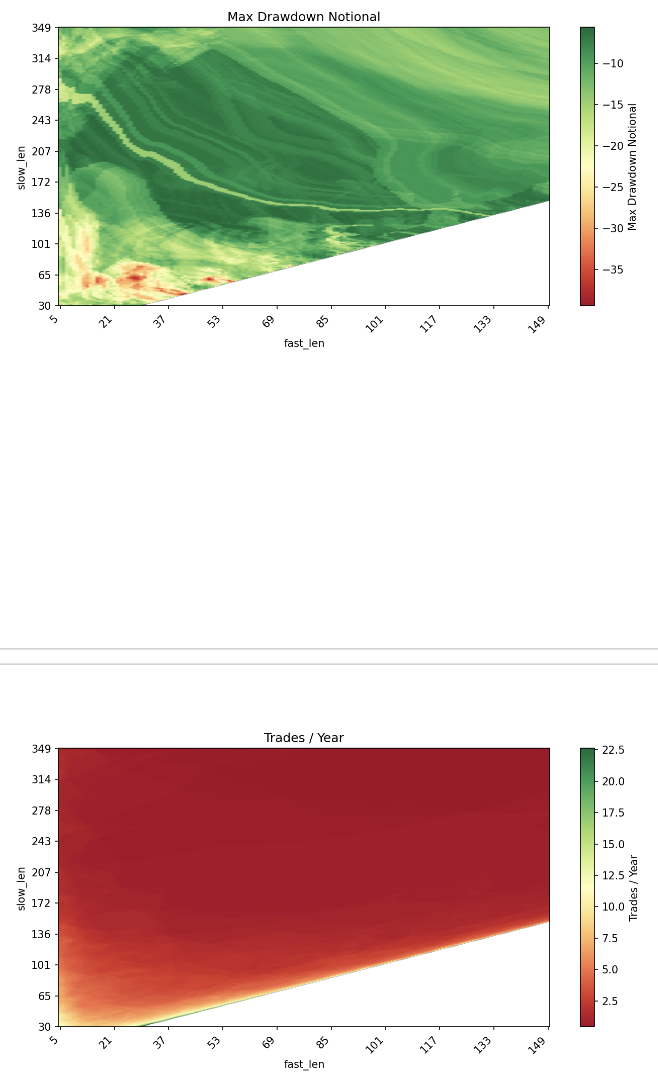
\includegraphics[width=\linewidth]{figures/opt/macross/ms2.png}
    \end{minipage}
    \hfill
    \begin{minipage}{0.49\textwidth}
        \centering
        \textbf{Synthetic mean}\\[0.2em]
        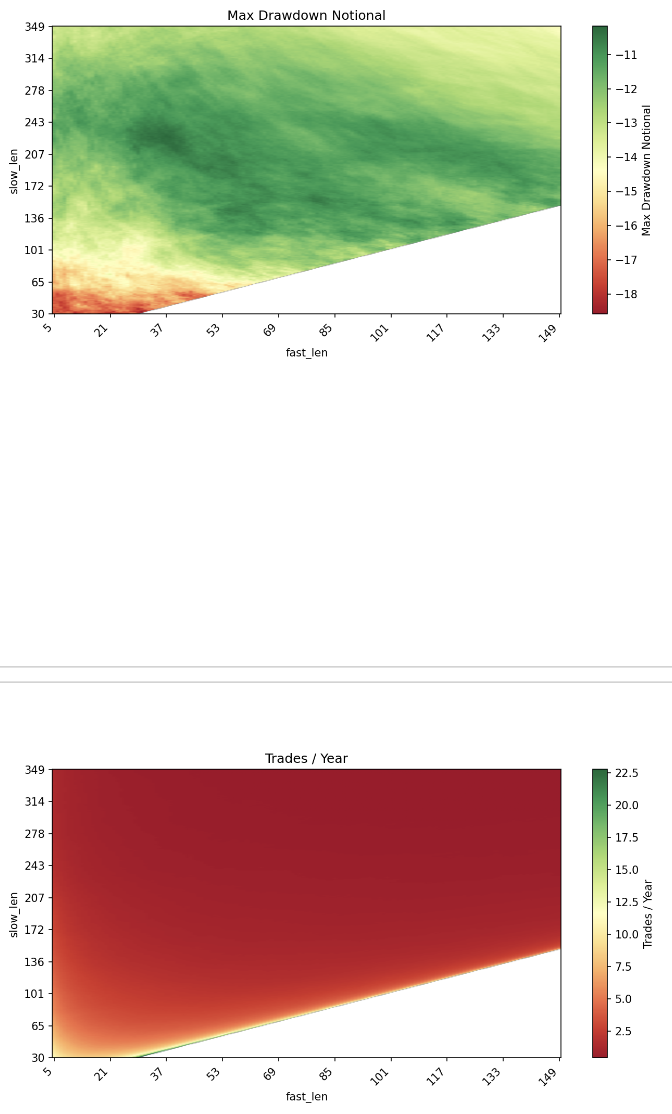
\includegraphics[width=\linewidth]{figures/opt/macross/syn_mas2.png}
    \end{minipage}

    \caption{Moving-average crossover: second metric panel over the fast/slow length grid.}
    \label{fig:mac-ms2}
    \label{fig:mac-syn-ms2}
\end{figure}

Both grids show the same main pattern. Results are weak when the fast and slow lengths are close,
because the strategy trades too often on small price moves. Results improve when the slow length is
larger, creating a broad stable area near \(slow\_len = 200\). From this region, I chose
\(fast\_len = 50\), \(slow\_len = 200\) for the benchmark configuration. For the synthetic
configuration, I kept the same slow length but chose a shorter fast length:
\(fast\_len = 35\), \(slow\_len = 200\).

\section{Standard-deviation mean-reversion optimization}

\subsection{Stop-loss stage}

As with the crossover strategy, the stop-loss percentage was optimized first, holding the
standard-deviation length and thresholds at their resting values (\(std\_len = 15\),
\(lower\_std\_thresh = -1.5\), \(upper\_std\_thresh = 1.5\)). Figure~\ref{fig:mrev-slpct} sweeps the
stop-loss percentage from 0\% to 60\% on the real historical IS period.

\begin{figure}[H]
    \centering
    
\includegraphics[width=0.85\textwidth]{figures/opt/mrev/slpct.png}
    \caption{Std MRev: metrics as a function of the stop-loss percentage, historical IS.}
    \label{fig:mrev-slpct}
\end{figure}

For this strategy, the stop-loss curve has a clearer structure. Net profit and Sharpe improve for small
stop-loss values, around 1\%--3\%, then deteriorate and eventually flatten once the stop is so wide that
it rarely triggers. That flat region is stable, but it is not useful: a mean-reversion trade should be
cut when the move keeps going against it. For this reason, the benchmark stop-loss was selected from the
early profitable region, giving \(slpct = 2.5\%\). This is a risk-control choice, not a pure
maximum-metric choice.

The same sweep was repeated on synthetic paths, holding the same resting values.
Figures~\ref{fig:mrev-syn-slpct-np}--\ref{fig:mrev-syn-slpct-sharpe} report the synthetic-path mean.

\begin{figure}[H]
    \centering

    \begin{minipage}{0.49\textwidth}
        \centering
        \textbf{Net profit}\\[0.2em]
        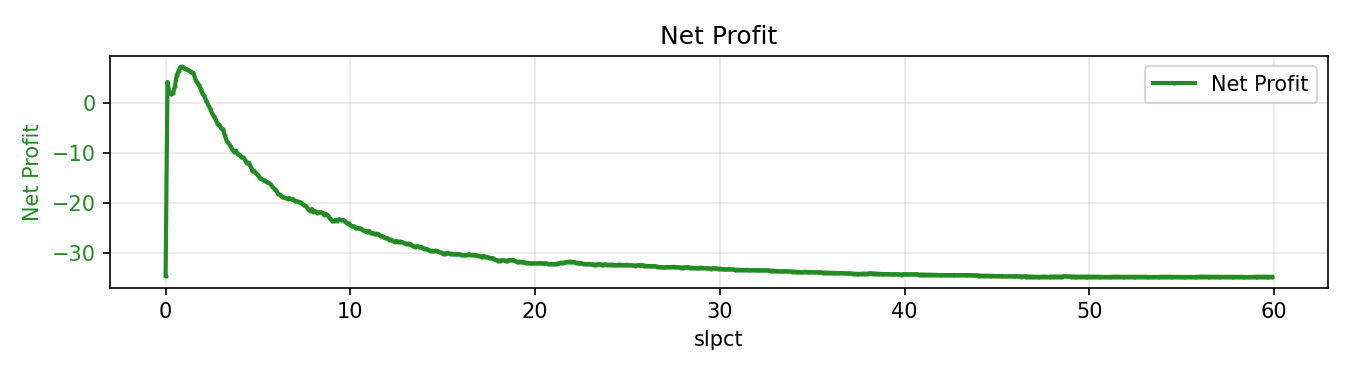
\includegraphics[width=\linewidth]{figures/opt/mrev/syn_slpct_net_profit.png}
    \end{minipage}
    \hfill
    \begin{minipage}{0.49\textwidth}
        \centering
        \textbf{Sharpe}\\[0.2em]
        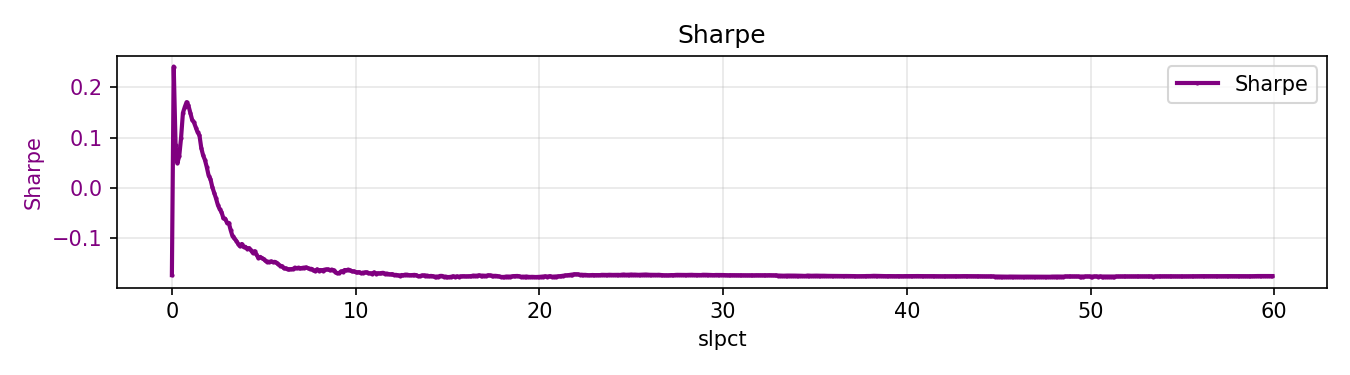
\includegraphics[width=\linewidth]{figures/opt/mrev/syn_slpct_sharpe.png}
    \end{minipage}

    \caption{Std MRev: stop-loss optimization, mean over synthetic paths.}
    \label{fig:mrev-syn-slpct-np}
    \label{fig:mrev-syn-slpct-sharpe}
\end{figure}

Averaging over synthetic paths removes most of the noise. The curve rises near the 1\% area and then
decays toward the same inactive-stop plateau. The best single point, \(slpct = 0.1\%\), is too isolated
to use directly. Using the same risk-control logic as above, the synthetic configuration uses
\(slpct = 2.0\%\).

\subsection{Length and linked threshold stage}

With the stop-loss fixed, I optimized the standard-deviation length together with one threshold level.
To avoid optimizing the length alone, but also avoid a three-parameter grid, the upper and lower
thresholds were linked symmetrically: one positive threshold for short entries and one negative
threshold of the same size for long entries.
Figure~\ref{fig:mrev-sllen1} compares the main historical-IS grid with the synthetic-path mean.
Figure~\ref{fig:mrev-sllen2} shows the trades/year surface for the historical-IS grid, since it helps
explain how the optimization process was interpreted. The synthetic version was very similar, so it is
not repeated here.

\begin{figure}[H]
    \centering

    \begin{minipage}{0.49\textwidth}
        \centering
        \textbf{Historical IS}\\[0.2em]
        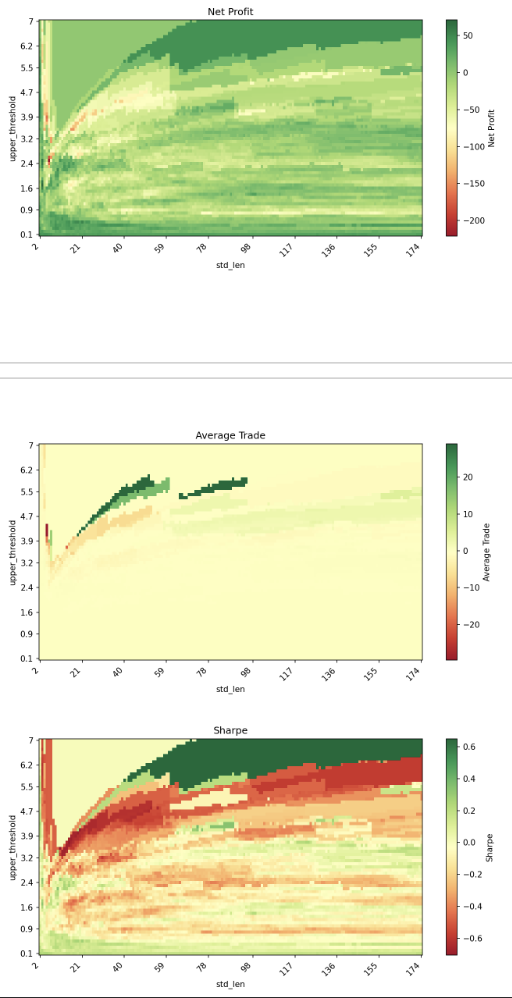
\includegraphics[width=\linewidth]{figures/opt/mrev/sllen_thresh.png}
    \end{minipage}
    \hfill
    \begin{minipage}{0.49\textwidth}
        \centering
        \textbf{Synthetic mean}\\[0.2em]
        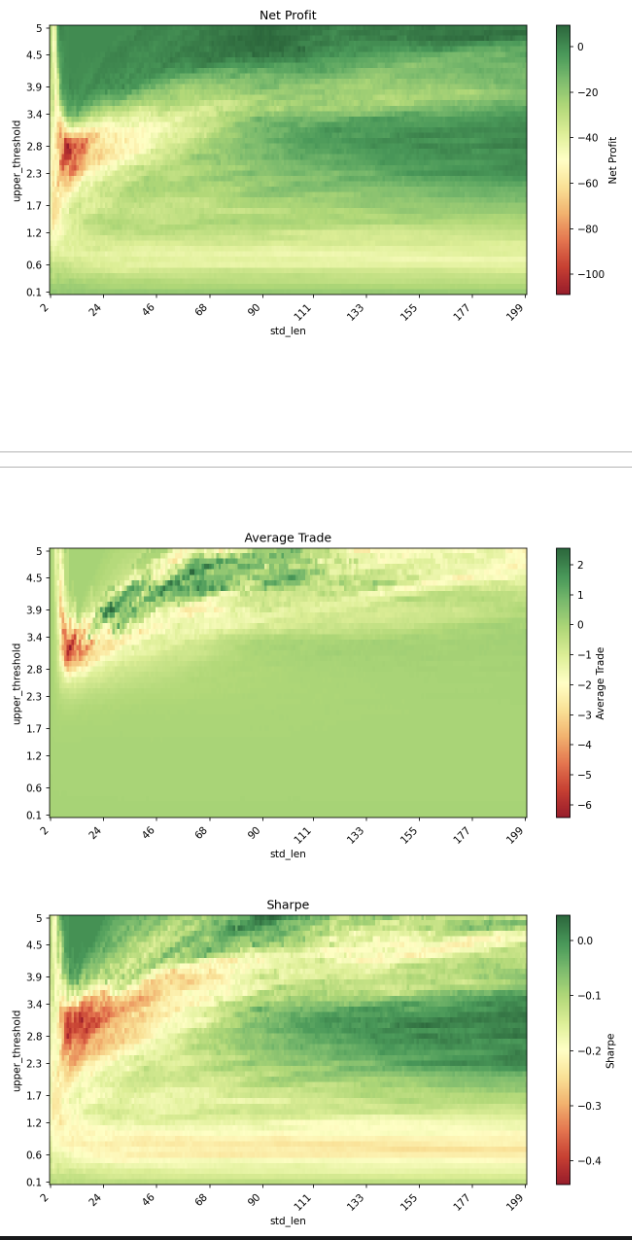
\includegraphics[width=\linewidth]{figures/opt/mrev/syn_slen_thresh.png}
    \end{minipage}

    \caption{Std MRev: first metric panel over the length/symmetric-threshold grid.}
    \label{fig:mrev-sllen1}
    \label{fig:mrev-syn-sllen}
\end{figure}

\begin{figure}[H]
    \centering
    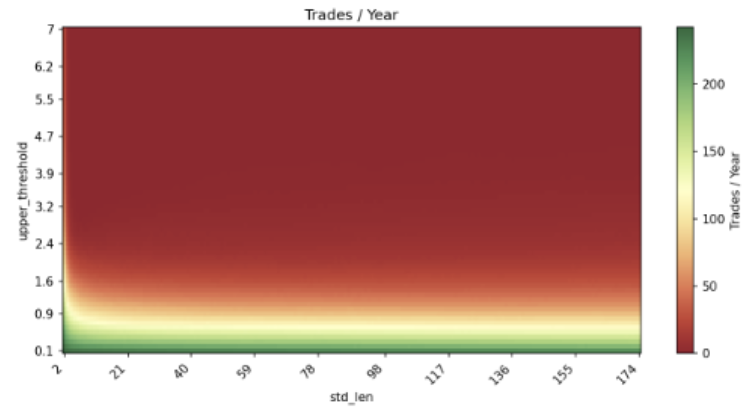
\includegraphics[width=0.85\textwidth]{figures/opt/mrev/show_in_5.7_instead_of_second_img.png}
    \caption{Std MRev: trades per year over the length/symmetric-threshold grid, historical IS.}
    \label{fig:mrev-sllen2}
\end{figure}

Very short standard-deviation lengths perform poorly because they react to almost every local move. In
the historical grid, performance becomes usable around 20--40 bars, so the benchmark configuration uses
\(std\_len = 20\) and a narrow symmetric threshold as the starting point. In the synthetic grid, the
stable area appears much later, around 100--150 bars, with a wider threshold. The synthetic
configuration therefore uses \(std\_len = 150\) and starts from a wider threshold. The symmetric
threshold is only an intermediate step; the final stage separates the upper and lower thresholds.

\subsection{Independent threshold stage}

Finally, the upper and lower thresholds were optimized independently, holding the standard-deviation
length and stop-loss at the values selected in the previous stages. Figure~\ref{fig:mrev-tt} compares
the main historical-IS grid at \(std\_len = 20\) with the synthetic-path mean at \(std\_len = 150\).
Figure~\ref{fig:mrev-syn-tt2} shows the trades/year surface to make the optimization process easier to
read. The benchmark and synthetic trades/year plots were very similar, so only this one is reported.

\begin{figure}[H]
    \centering

    \begin{minipage}{0.49\textwidth}
        \centering
        \textbf{Historical IS}\\[0.2em]
        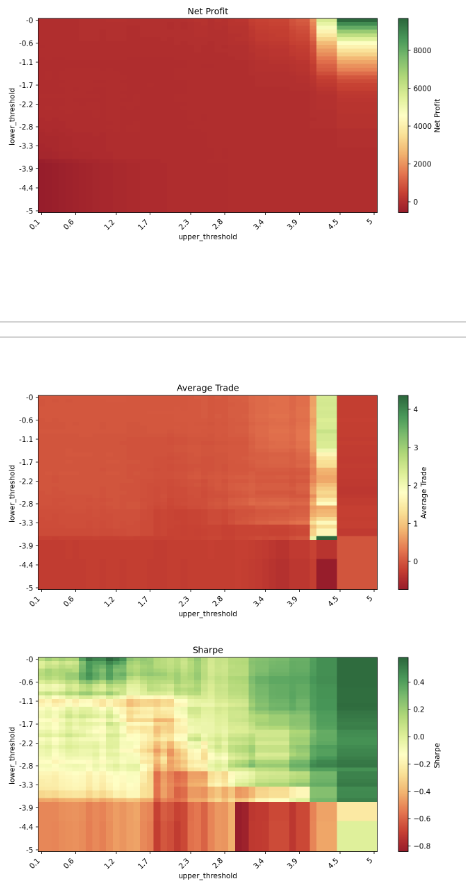
\includegraphics[width=\linewidth]{figures/opt/mrev/thresh_thresh.png}
    \end{minipage}
    \hfill
    \begin{minipage}{0.49\textwidth}
        \centering
        \textbf{Synthetic mean}\\[0.2em]
        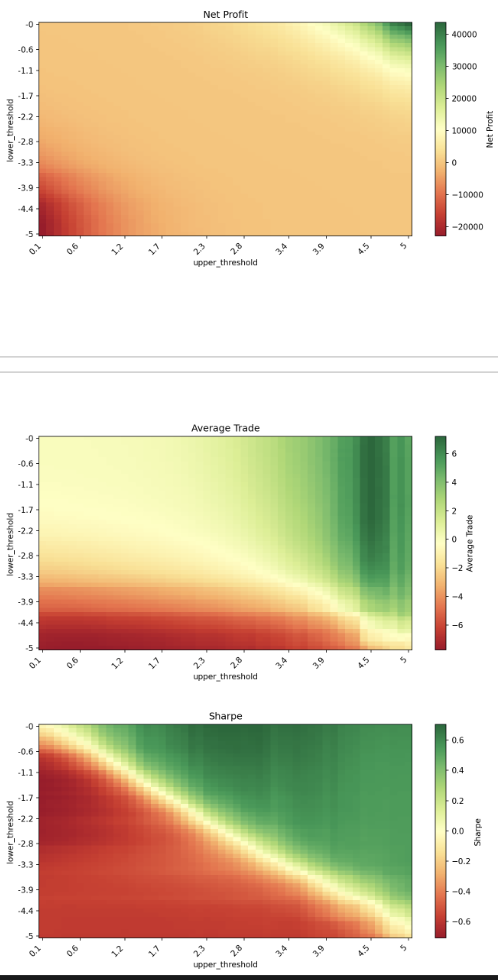
\includegraphics[width=\linewidth]{figures/opt/mrev/syn_thresh_thresh.png}
    \end{minipage}

    \caption{Std MRev: first metric panel over the independent upper/lower threshold grid.}
    \label{fig:mrev-tt}
    \label{fig:mrev-syn-tt1}
\end{figure}

Figure~\ref{fig:mrev-tt} is one of the clearest examples of why the synthetic-path mean is useful. In
particular, the Sharpe surface is much smoother on the synthetic side. Averaging across paths appears to
cancel part of the single-path noise and makes the stable region easier to see, although the two panels
come from the parameter settings used in each workflow.

\begin{figure}[H]
    \centering
    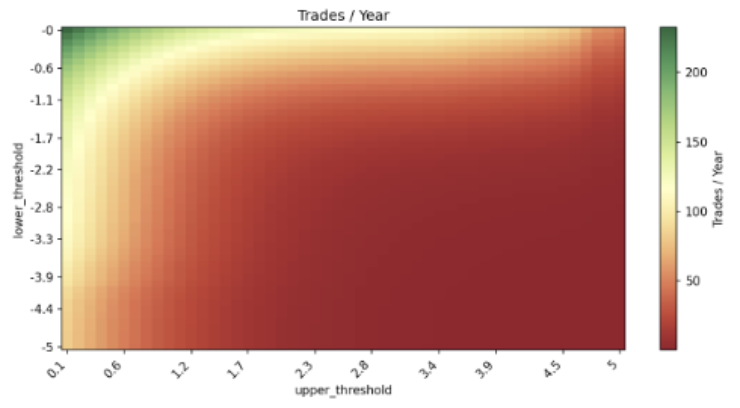
\includegraphics[width=0.85\textwidth]{figures/opt/mrev/show_in_5.9.png}
    \caption{Std MRev: trades per year over the independent upper/lower threshold grid.}
    \label{fig:mrev-syn-tt2}
\end{figure}

The independent-threshold grids show that the symmetric rule is not ideal. Performance improves when
the lower threshold is kept close to zero and the upper threshold is wider. The final benchmark
thresholds are \(upper\_std\_thresh = 1.0\), \(lower\_std\_thresh = -0.35\). The final synthetic
thresholds are \(upper\_std\_thresh = 3.0\), \(lower\_std\_thresh = -0.30\). In both cases, the strategy
becomes more sensitive to downside moves than upside moves.

\section{Selected parameters}

Table~\ref{tab:selected-params} summarizes the selected parameters. These configurations are fixed and
then evaluated on the real OOS period in the following chapter.

\begin{table}[H]
    \centering
    \begin{tabular}{lllll}
        \toprule
        Strategy & Method & Parameters & slpct & Other \\
        \midrule
        MA Cross & Benchmark & fast=50, slow=200 & disabled & -- \\
        MA Cross & Synthetic & fast=35, slow=200 & disabled & -- \\
        Std MRev & Benchmark & std\_len=20 & 2.5\% & upper=1.0, lower=-0.35 \\
        Std MRev & Synthetic & std\_len=150 & 2.0\% & upper=3.0, lower=-0.30 \\
        \bottomrule
    \end{tabular}
    \caption{Final selected parameters per strategy and optimization method.}
    \label{tab:selected-params}
\end{table}

Both methods use the same optimization process: parameters are chosen from robust grid regions rather
than isolated peaks. The difference is the optimization data: the benchmark uses the real historical IS
period, while the synthetic method uses the mean result across synthetic IS paths. The real test is the
next step: comparing IS-to-OOS deterioration and checking whether the synthetic method reduces it.
